\documentclass{VUMIFPSkursinis}
\usepackage{algorithmicx}
\usepackage{algorithm}
\usepackage{algpseudocode}
\usepackage{amsfonts}
\usepackage{amsmath}
\usepackage{bm}
\usepackage{caption}
\usepackage{color}
\usepackage{float}
\usepackage{graphicx}
\usepackage{listings}
\usepackage{subfig}
\usepackage{wrapfig}


% Titulinio aprašas
\university{Vilniaus universitetas}
\faculty{Matematikos ir informatikos fakultetas}
\department{Programų sistemų katedra}
\papertype{Kursinis darbas}
\title{Mobiliųjų programų testavimas remiantis TMMi modeliu.}
\titleineng{TMMi model based mobile application testing.}
\status{3 kurso 4 grupės studentas}
\author{Ričardas Mikelionis}
\supervisor{dr. Vytautas Valaitis}
\date{Vilnius – \the\year}

% Nustatymai
\setmainfont{Palemonas}   % Pakeisti teksto šriftą į Palemonas (turi būti įdiegtas sistemoje)
\bibliography{bibliografija}

\begin{document}
\maketitle

\cleardoublepage
\pagenumbering{gobble}
\tableofcontents
\cleardoublepage
\pagenumbering{arabic}

\sectionnonum{Įvadas}
Nuo 2007, kai buvo pristatytas pirmasis iPhone jau praėjo kiek daugiau nei dešimt metų. Šio mobiliojo įrenginio, išmaniojo telefono (angl. Smartphone), pristatymas sukrėtė ir iš esmės pakeitė mobiliųjų kompiuterių rinką. Iki tol asmeniniai skaitmeniai asistentai (angl. PDA personal digital asistant) buvo nei prieinami, nei labai naudingi įprastam vartotojui, todėl juos turėjo keletas verslo pasaulio žmonių, o paprastas vartotojas su savimi nešiojosi krūvą skirtingą funkcionalumą atliekančių prietaisų: MP3 grotuvų, Fotoaparatų, nešiojamųjų kompiuterių, telefonų. iPhone žadėjo delne telpantį kompiuterį kiekvienam už prieinamą kainą, ir savo pažadą įvykdė. Vienas po kito ėmė rastis  mobiliosios operacinės sistemos, turėjusios tiesiogiai konkuruoti su iPhone naudojama iOS,  kaip PalmOS, Symbian, Windows 7 mobile, vėliau tapusi 8 ir 8.1 bei Android. Mobiliųjų kompiuterių bei telefonų rinką apėmė ir užplūdo krūvos prieinamų įrenginių, kurie su kiekviena nauja laida savo skaičiavimo sugebėjimais artėja arčiau ir arčiau to ką gali atlikti staliniai kompiuteriai, ir iš pažiūros 2017 metų išmanusis įrenginys savo specifikacijomis „ant popieriaus“ jau seniai pranoko 2007 metų kompiuterį.

Nors šiandien iš gausauss operacinių sistemų pasirinkimo rinkoje iš esmės išlikę tik dvi: iOS ir Android, tačiau  išmaniųjų prietaisų populiarumas toli gražu neblėsta. 2016 metais pasaulyje jau buvo apie 2.1 mlrd. išmaniųjų telefonų naudotojų, o iki 2020 planuojama, jog šis skaičius sieks 2.87 mlrd.\cite {statista.com}. Esant didžulei įrenginių paklausai proporcingai kyla poreikis ir programinei įrangai pritaikytai šiems įrenginiams - mobiliosioms programoms.

Šio darbu siekiama pateikti esminius skirtumus tarp įprastų darbastalio (angl. desktop) bei internetinių (angl. Web) programų ir mobiliųjų programų skirtų išmaniesiems įrenginiams kokybės užtikrinimo. Šio darbo tikslas - išanalizavus dabar rinkoje esančius mobiliųjų programų kokybės užtikrinimo įrankius, išskirti problemines mobiliųjų programų kokybės užtikrinimo sritis.



\section{Mobiliųjų programų kokybė.}

2013 metais atliktas tyrimas \cite {compuware.com} rodo, jog 79\% išmaniųjų telefonų naudotojų išbando atsisiųstą programėlę tik kartą prieš ištrindami. Didelė to priežastis yra žemesnė mobiliųjų programų kokybė palyginus su tuo ką vartotojai yra įpratę matyti savo naršyklėse, ar darbastalio programose. Išmaniųjų telefonų naudotojai yra pratę prie nemokamos ar žymiai mažiau kainuojančios programinės įrangos, kuri gauna nuolatinius atnaujinimus. (Pvz.: Adobe photoshop express iOS 0eur., Adobe Photoshop Windows 10 290eur./m. \cite{adobe.com}). Kyla kainų dilema: norint palaikyti žemas kainas rinkoje reikia mažinti kainas ir kūrimo procese. Tai dažnai daroma taupant laiką, kur ir nukenčia kokybės užtikrinimo procesai.

Į mobiliųjų programų kūrimą vis dar žiūrima taip pat, kaip į interneto programų (angl. WEB application) ar darbastalio programų kūrimą, neįžvelgiant esminių skirtumų tarp šių dviejų programinės įrangos kūrimo procesų. Didžiulė įrenginių variacijų gausa, ir iš esmės išsiskiriantys naudojimosi mobiliąja programine įranga įpročiai turėtų versti kūrėjus į mobiliųjų programų kūrimą žvelgti kitaip.

\subsection{Mobiliųjų programų kūrimo proceso skirtumai.}
M. Satyanarayanan dar 1996-aisiais savo straipsnyje apie mobiliuosius kompiuterius puikiai aibrėžė esmines sritis, kurios išskiria mobiliuosius įrenginius nuo stacionariųjų. Išskirtos keturios sritys: riboti skaičiavimo ištekliai (angl. limited computing resources), apsauga ir pažeidžiamumas, galia (angl. performance) ir patikimumas bei riboti energijos ištekliai. \cite{Satyanarayanan:1996:FCM:248052.248053} Remiantis šiomis išskirtinumo sritimis galima pradėti išskirti esmines problemines sritis, į kurias derėtų atkreipti dėmesį kuriant bei testuojant programinę įrangą skirtą mobiliesiems įrenginiams.

\subsubsection{Skirsnis}
\subsubsubsection{Straipsnis}
\subsubsection{Skirsnis}
\section{Skyrius}
\subsection{Poskyris}
\subsection{Poskyris}

\sectionnonum{Rezultatai ir išvados}
Rezultatų ir išvadų dalyje turi būti aiškiai išdėstomi pagrindiniai darbo
rezultatai (kažkas išanalizuota, kažkas sukurta, kažkas įdiegta) ir pateikiamos
išvados (daromi nagrinėtų problemų sprendimo metodų palyginimai, teikiamos
rekomendacijos, akcentuojamos naujovės).

\printbibliography[heading=bibintoc]  % Šaltinių sąraše nurodoma panaudota
% literatūra, kitokie šaltiniai. Abėcėlės tvarka išdėstomi darbe panaudotų
% (cituotų, perfrazuotų ar bent paminėtų) mokslo leidinių, kitokių publikacijų
% bibliografiniai aprašai.  Šaltinių sąrašas spausdinamas iš naujo puslapio.
% Aprašai pateikiami netransliteruoti. Šaltinių sąraše negali būti tokių
% šaltinių, kurie nebuvo paminėti tekste.

% \sectionnonum{Sąvokų apibrėžimai}
\sectionnonum{Santrumpos}
Sąvokų apibrėžimai ir santrumpų sąrašas sudaromas tada, kai darbo tekste
vartojami specialūs paaiškinimo reikalaujantys terminai ir rečiau sutinkamos
santrumpos.

\appendix  % Priedai
% Prieduose gali būti pateikiama pagalbinė, ypač darbo autoriaus savarankiškai
% parengta, medžiaga. Savarankiški priedai gali būti pateikiami ir
% kompaktiniame diske. Priedai taip pat numeruojami ir vadinami. Darbo tekstas
% su priedais susiejamas nuorodomis.

\section{Neuroninio tinklo struktūra}
\begin{figure}[H]
    \centering
    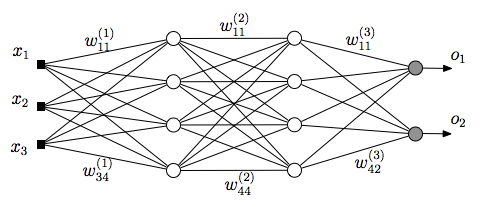
\includegraphics[scale=0.5]{img/MLP}
    \caption{Paveikslėlio pavyzdys}
    \label{img:mlp}
\end{figure}


\section{Eksperimentinio palyginimo rezultatai}
% tablesgenerator.com - converts calculators (e.g. excel) tables to LaTeX
\begin{table}[H]\footnotesize
  \centering
  \caption{Lentelės pavyzdys}
  {\begin{tabular}{|l|c|c|} \hline
    Algoritmas & $\bar{x}$ & $\sigma^{2}$ \\
    \hline
    Algoritmas A  & 1.6335    & 0.5584       \\
    Algoritmas B  & 1.7395    & 0.5647       \\
    \hline
  \end{tabular}}
  \label{tab:table example}
\end{table}

\end{document}
